\section{Overview}
\label{sec:overview}%

The Best Bike Paths (BBP) system follows a client-server architecture that separates the mobile client application from the backend server infrastructure. The following diagram provides a high-level overview of the system architecture and the interactions between its main components.

\begin{figure}[H]
    \begin{center}
        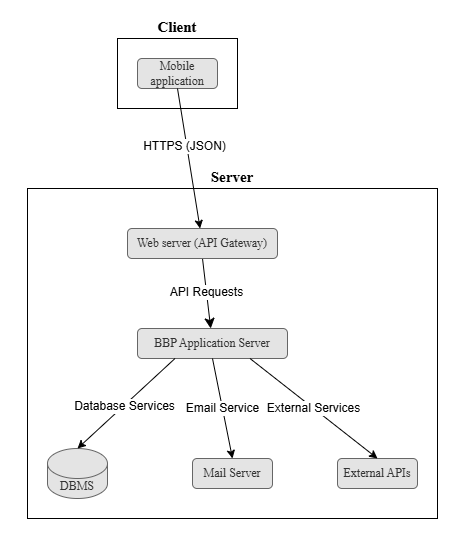
\includegraphics[width=0.6\linewidth]{Images/Diagrams/ArchitectureOverview.png}
        \caption{Architecture Overview Diagram for Best Bike Paths System}
        \label{fig:architecture_overview}%
    \end{center}
\end{figure}

The architecture is divided into two main logical sections: the Client and the Server. 

\subsection{Client Side}
The client side consists of the Mobile Application, available for both iOS and Android platforms. This application serves as the primary interface for users, allowing them to interact with the BBP system. The mobile application communicates with the server using the HTTPS protocol, exchanging data in JSON format.

\subsection{Server Side}
The server side is composed of several interconnected components that work together to process requests and manage system operations:

\begin{itemize}
    \item \textbf{Web Server (API Gateway):} This component receives HTTPS requests from the mobile application and acts as an API Gateway, handling request routing, authentication, and initial request validation. The API Gateway forwards validated API requests to the BBP Application Server.
    
    \item \textbf{BBP Application Server:} This component processes API requests received from the Web Server and coordinates interactions with various backend services. The BBP Application Server handles all core functionalities including user management, trip recording, path management, automated detection, path search, information merging, and rating services.
    
    \item \textbf{DBMS (Database Management System):} The database server stores all persistent data required by the system, including user profiles and authentication data, trip recordings and statistics, path information with status and obstacles, ratings and reviews, and system configuration data. 
    
    \item \textbf{Mail Server:} This component handles all email-related operations required by the system, such as sending verification emails, password recovery emails, and other notification emails to users.
    
    \item \textbf{External APIs:} This component represents the integration with external third-party services, such as weather data APIs (for enriching trip data with meteorological information) and map service APIs (for displaying routes and geographic information).
\end{itemize}

The architecture ensures clear separation of concerns, with each component having well-defined responsibilities. Communication between components follows a request-response pattern, and the use of HTTPS and JSON ensures secure and platform-independent data exchange.

\section{Component View}
\label{sec:component_view}%

The Component View describes the \textbf{logical structure} and \textbf{functional organization} of the BBP system. This view focuses on what components exist, what responsibilities each component has, and how they interact logically, independent of physical deployment considerations.

The BBP system is composed of several key components organized in a layered architecture. The following diagram illustrates the main components and their relationships:

\begin{figure}[H]
    \begin{center}
        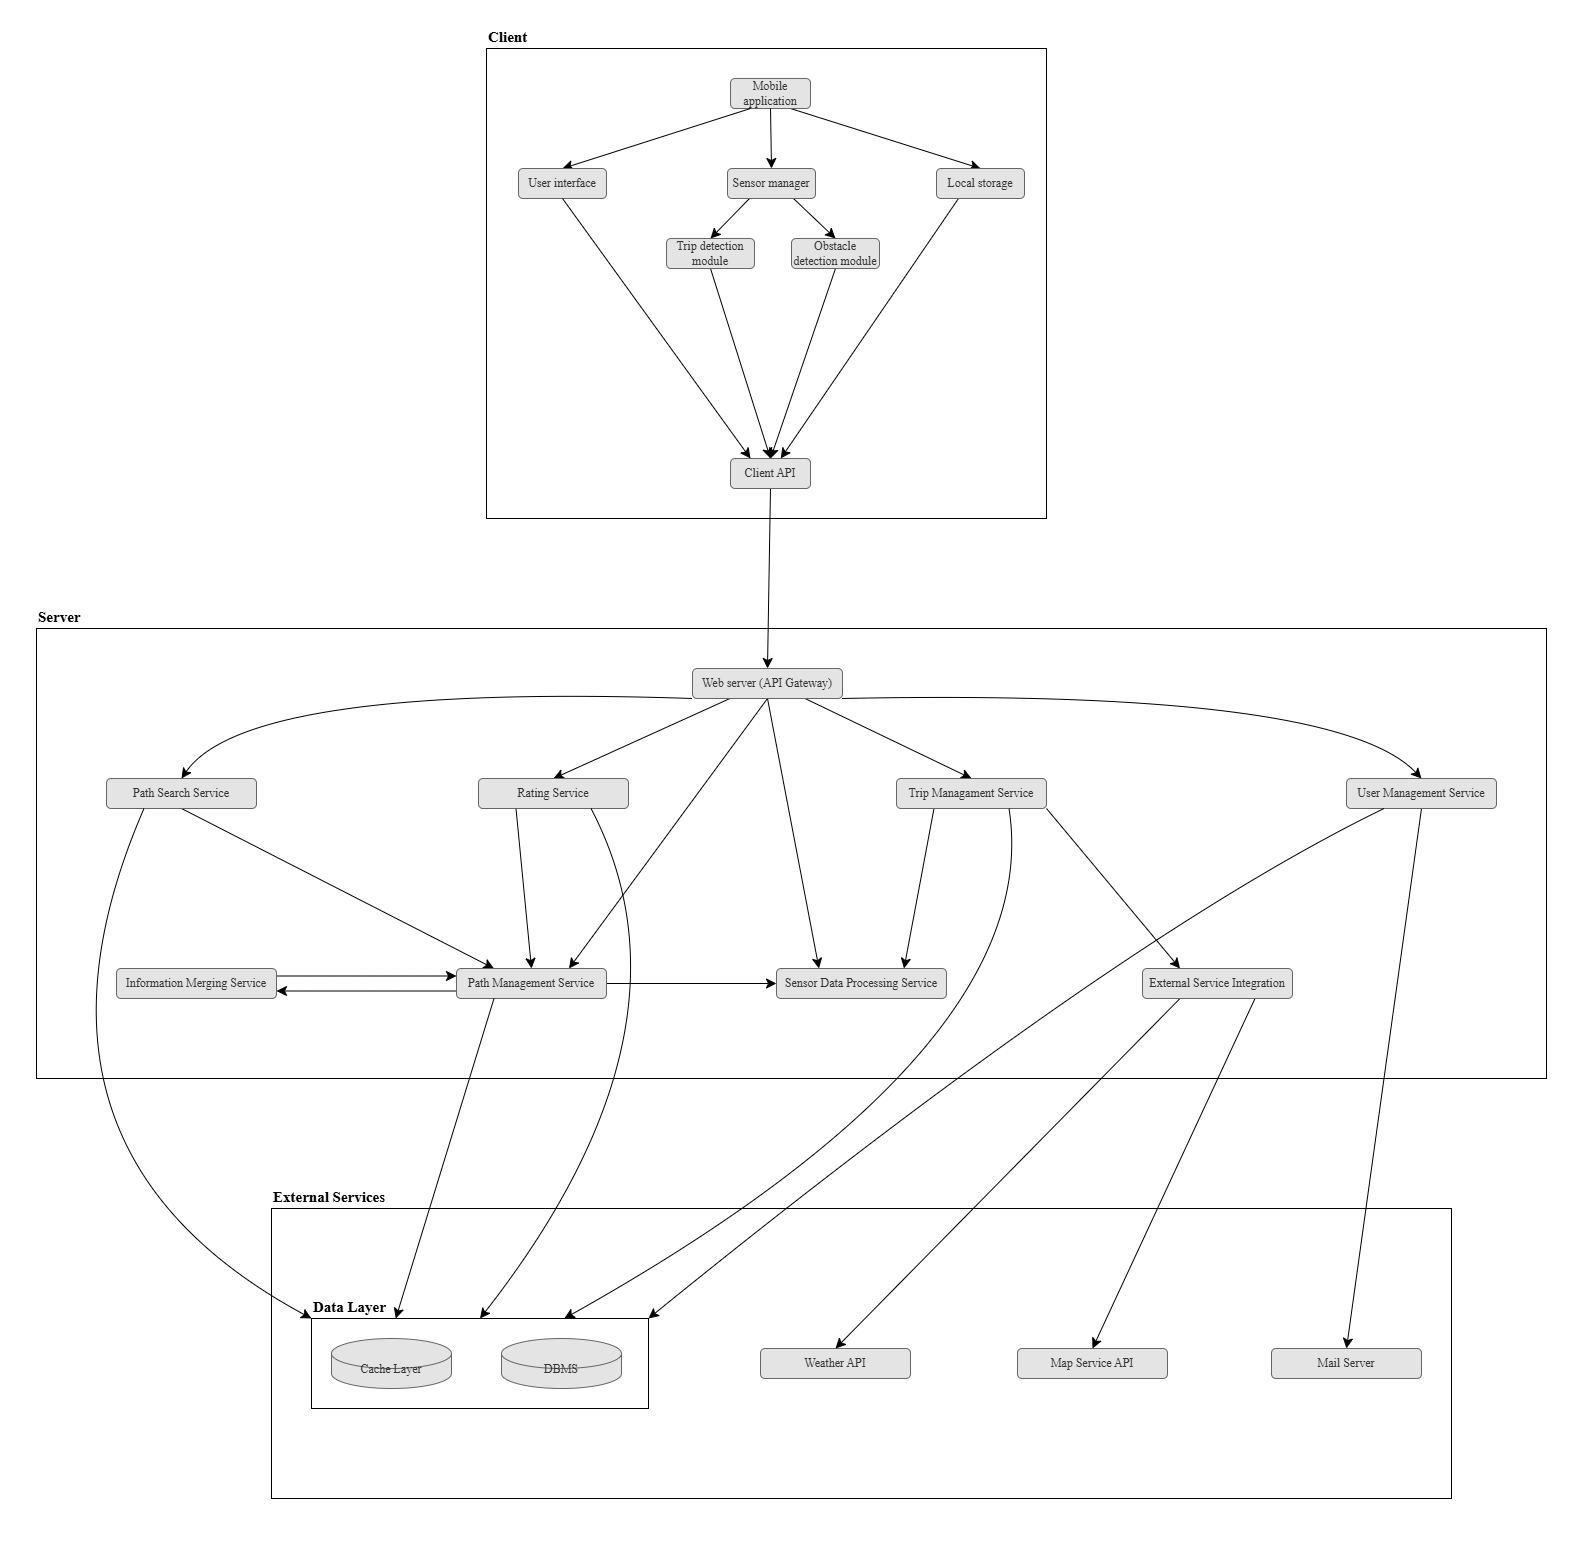
\includegraphics[width=1.0\linewidth]{Images/Diagrams/ComponentViewDiagram.png}
        \caption{Component Diagram for Best Bike Paths System}
        \label{fig:component_diagram}%
    \end{center}
\end{figure}

\subsection{Client-Side Components}

\subsubsection{Mobile Application}
The mobile application is the primary interface for users and consists of:

\begin{itemize}
    \item \textbf{User Interface Module:} Handles all user interactions, displays maps, paths, trips, and statistics.
    \item \textbf{Sensor Manager:} Manages access to device sensors (GPS, accelerometer, gyroscope) and collects sensor data during trips.
    \item \textbf{Local Storage:} Provides offline capabilities by caching data locally.
    \item \textbf{Client API:} Handles all communication with the backend through API calls.
    \item \textbf{Trip Detection Engine:} Performs lightweight, real-time analysis of GPS speed data to detect when a user begins cycling. This component runs continuously in the background with minimal battery consumption, using simple pattern recognition algorithms to identify cycling activity. 
    \item \textbf{Obstacle Detection Module:} Performs real-time analysis of accelerometer and gyroscope data to identify sudden anomalies that may indicate obstacles such as potholes. This component monitors sensor readings continuously during active trips, using threshold based algorithms to detect significant vibrations or device movements that deviate from normal cycling patterns.
\end{itemize}

\subsection{Server-Side Components}

The server-side architecture is composed of multiple specialized services that work together to handle the core business logic of the BBP system. Each service is designed with a specific domain responsibility, ensuring clear separation of concerns.

\subsubsection{API Gateway}
The \textbf{API Gateway} acts as the \textbf{single entry point} for all client requests, serving as a critical layer between the mobile applications and the backend services. 

The gateway handles \textbf{request routing} by analyzing the request path and method to determine which service should process it. 

Additionally, the gateway enforces \textbf{security policies} by performing \textbf{authentication and authorization} checks, ensuring that only authorized users can access protected resources. It also implements \textbf{validation} of incoming requests to ensure they conform to expected formats and contain required data.

\subsubsection{User Management Service}
The \textbf{User Management Service} is responsible for all aspects of \textbf{user account lifecycle} and \textbf{authentication} within the system. 

This service handles the complete \textbf{user registration process}, including validation of user-provided information and coordination with the Mail Server to send \textbf{verification emails}. Once users are registered, the service manages their authentication by processing \textbf{login requests} and creating \textbf{secure session tokens} that enable subsequent authenticated requests. 

The service also provides \textbf{password recovery} functionality, allowing users to reset their passwords through a secure process that involves email verification. Beyond authentication, the service maintains \textbf{user profile information}, enabling users to update their personal details, preferences, and account settings. 

All user-related data is \textbf{securely stored and managed}, with proper \textbf{encryption} and \textbf{access controls} to protect sensitive information.

\subsubsection{Trip Management Service}
The Trip Management Service manages all operations related to cycling trips recorded by users. 

This service supports both \textbf{manual trip recording}, where users explicitly enter trip information, and \textbf{automatic trip detection}, where the system identifies cycling activity based on sensor data patterns. 

When trips are recorded, the service calculates comprehensive \textbf{statistics} including total distance covered, average speed, duration, and elevation changes when available. The service maintains a complete \textbf{history} of all trips for each user, enabling users to review their past cycling activities and track their progress over time. To enrich trip data, the service integrates with \textbf{external weather APIs} to retrieve meteorological information that were present during the trip.

\subsubsection{Path Management Service}
The \textbf{Path Management Service} is the \textbf{central component} for managing bike path information within the system. 

It handles the \textbf{creation and maintenance of path data}, supporting both \textbf{manual entry} by users and \textbf{automatic path detection} from GPS data collected during trips. The service manages \textbf{path status information}, allowing users to report and update the condition of paths (e.g., optimal, medium, sufficient, or requiring maintenance). It also tracks \textbf{obstacles} such as potholes that are detected on paths, storing their \textbf{locations and characteristics}. 

When users create or update path information, the service provides functionality to make paths \textbf{publishable}, making them available to the broader community of users. The service also handles \textbf{path data retrieval}, serving path information to other services such as the Path Search Service when users query for available routes.

\subsubsection{Sensor Data Processing Service}
The \textbf{Sensor Data Processing Service} performs comprehensive, \textbf{server-side processing} of raw sensor data collected from mobile devices during cycling activities. Unlike the lightweight detection modules in the mobile application that perform real-time, battery-efficient initial detection, this service executes more sophisticated \textbf{signal processing algorithms} that require additional computational resources available on the server. The purpose of this service is to improve the \textbf{accuracy and reliability} of the final path and obstacle data compared to the initial client-side detection, which is then presented to users for confirmation before being made available to the community.

The service handles two main types of sensor data processing:

\begin{itemize}
    \item \textbf{GPS Coordinate Streams Processing:} The service receives complete \textbf{GPS coordinate streams} collected during trips and applies \textbf{path reconstruction algorithms} to convert discrete location points into accurate, continuous route representations. The service also performs \textbf{outlier detection} to identify and remove erroneous GPS points that deviate significantly from the expected route, ensuring that the reconstructed path accurately represents the actual route followed by the user.
    \item \textbf{Obstacle Detection Processing:} For obstacle detection, the service performs detailed analysis of \textbf{accelerometer and gyroscope data} using \textbf{statistical filtering methods} that go beyond the simple threshold-based detection performed on the client. It \textbf{correlates obstacle candidates} identified by the mobile application with \textbf{precise GPS locations}, enabling accurate spatial positioning of detected obstacles. It uses \textbf{statistical analysis} to distinguish real obstacles from \textbf{transient sensor noise}, filtering out anomalies that do not meet established criteria for obstacle characteristics. The service \textbf{validates obstacle detections} by checking consistency with cycling patterns, such as verifying that detected obstacles align with the user's speed and movement direction at the time of detection.
\end{itemize}

\subsubsection{Path Search Service}
The \textbf{Path Search Service} provides the functionality for users to \textbf{discover and visualize} bike paths between specified origin and destination points. 

When a user requests a path search, the service executes \textbf{path finding algorithms} that identify all available routes connecting the origin and destination, considering all the paths stored in the system. For each identified path, the service calculates a \textbf{comprehensive score} that evaluates multiple factors including the path's current status (optimal, medium, sufficient, or requiring maintenance), the \textbf{presence and severity of obstacles}, and the path's \textbf{effectiveness} in reaching the destination efficiently. 

Based on these scores, the service \textbf{ranks all available paths}, presenting the most suitable options first. The service also prepares data for \textbf{map visualization}, formatting path information in a way that enables the mobile application to display routes clearly on interactive maps.

\subsubsection{Information Merging Service}
The \textbf{Information Merging Service} handles the complex task of \textbf{consolidating path information} provided by multiple users, ensuring that the system maintains accurate and up to date path data despite conflicting reports. 

When multiple users provide information about the same path, the service collects all \textbf{publishable information} and analyzes it to determine the most accurate representation. The service implements \textbf{conflict resolution strategies} that consider both the \textbf{freshness of information} and the \textbf{consensus among users}. 

When merging \textbf{path status information}, the service evaluates all reported statuses and selects the most appropriate one based on \textbf{recency} and the \textbf{number of confirming reports}. Similarly, when consolidating \textbf{obstacle information}, the service combines reports from different users, removes duplicates, and prioritizes recent and confirmed obstacle detections.

\subsubsection{Rating Service}
The \textbf{Rating Service} manages the \textbf{community-driven rating and review system} that allows users to provide feedback about bike paths. 

This service enables registered users to \textbf{create ratings} for paths they have used, allowing them to assign \textbf{numerical scores} and optionally provide \textbf{written comments} describing their experience. Users can also \textbf{update their existing ratings} if their opinion about a path changes over time. 

The service maintains a comprehensive collection of all ratings and reviews for each path, organizing them \textbf{chronologically} and by \textbf{rating value}. It calculates \textbf{overall path ratings} by aggregating individual user ratings, providing a \textbf{community consensus view} of path quality. 

When users \textbf{request to view ratings} for a path, the service \textbf{retrieves and filters reviews} based on various criteria such as date range, rating value, or specific keywords, helping users find the most relevant feedback.

\subsubsection{External Service Integration}
The \textbf{External Service Integration} component manages all interactions with \textbf{third-party services} that provide additional functionality to the BBP system. 

This component integrates with \textbf{weather data APIs} to retrieve meteorological information that enriches trip data, providing users with context about weather conditions during their cycling activities. It also integrates with \textbf{map service APIs} that provide geographic data, route visualization capabilities, and mapping functionality essential for displaying paths to users. 

The component implements \textbf{robust error handling mechanisms} to gracefully manage situations where external services are temporarily unavailable, ensuring that the application continues to function even when external dependencies fail. 

\subsection{Data Layer Components}

The data layer provides persistent storage for all system data, ensuring data integrity, availability, and efficient retrieval. This layer is fundamental to the system's operation, as it maintains the state of all entities and relationships that define the BBP platform.

\subsubsection{Database Management System}
The \textbf{Database Management System} serves as the \textbf{central repository} for all persistent data required by the BBP system. 

It stores comprehensive \textbf{user data} including user profiles with personal information, preferences, and account settings, as well as \textbf{authentication credentials} that are securely hashed and protected. The database maintains detailed \textbf{trip data}, preserving complete records of all cycling trips including GPS coordinates, timestamps, calculated statistics such as distance and average speed, and associated metadata. 

\textbf{Path data} is extensively stored, including complete route information with origin and destination points, path status information that reflects current conditions, and detailed obstacle data with precise locations and characteristics. The system also maintains all \textbf{rating and review data}, storing user-generated feedback including numerical scores, written comments, and timestamps that enable chronological organization and filtering. 

\subsubsection{Cache Layer}
The system implements a \textbf{cache layer} to improve performance and reduce database load. The cache stores frequently accessed data such as popular paths, user session information, and path search results. This layer uses in-memory storage to provide fast data retrieval, significantly reducing response times for common queries and enhancing the overall system performance.

\subsection{Component Dependencies}

The following table summarizes the key dependencies between components, showing which components depend on others:

\begin{table}[H]
\centering
\small
\begin{tabularx}{\textwidth}{|l|X|}
\hline
\textbf{Component} & \textbf{Dependencies} \\
\hline
Mobile Application & User Interface Module, Local Storage, Sensor Manager \\
\hline
User Interface Module & Client API \\
\hline
Sensor Manager & Trip Detection Module, Obstacle Detection Module \\
\hline
Trip Detection Module & Client API \\
\hline
Obstacle Detection Module & Client API \\
\hline
Local Storage & Client API \\
\hline
Client API & Web Server (API Gateway) \\
\hline
Web Server (API Gateway) & Path Search Service, Rating Service, Trip Management Service, User Management Service, Sensor Data Processing Service \\
\hline
User Management Service & Mail Server, Data Layer \\
\hline
Trip Management Service & Sensor Data Processing Service, External Service Integration, Data Layer \\
\hline
Path Management Service & Sensor Data Processing Service, Information Merging Service, Data Layer \\
\hline
Path Search Service & Path Management Service, Data Layer \\
\hline
Rating Service & Path Management Service, Data Layer \\
\hline
External Service Integration & Weather API, Map Service API \\
\hline
\end{tabularx}
\caption{Component Dependencies Matrix}
\label{tab:component_dependencies}
\end{table}

\section{Deployment View}
\label{sec:deployment_view}%

The Deployment View describes the \textbf{physical infrastructure} and \textbf{deployment architecture} of the BBP system. This view focuses on where components are deployed, what hardware and infrastructure resources are required, and how the system is distributed across physical nodes, servers, and devices.

The deployment architecture follows a distributed client-server model. The following diagram shows how components are deployed across different nodes:

\begin{figure}[H]
    \begin{center}
        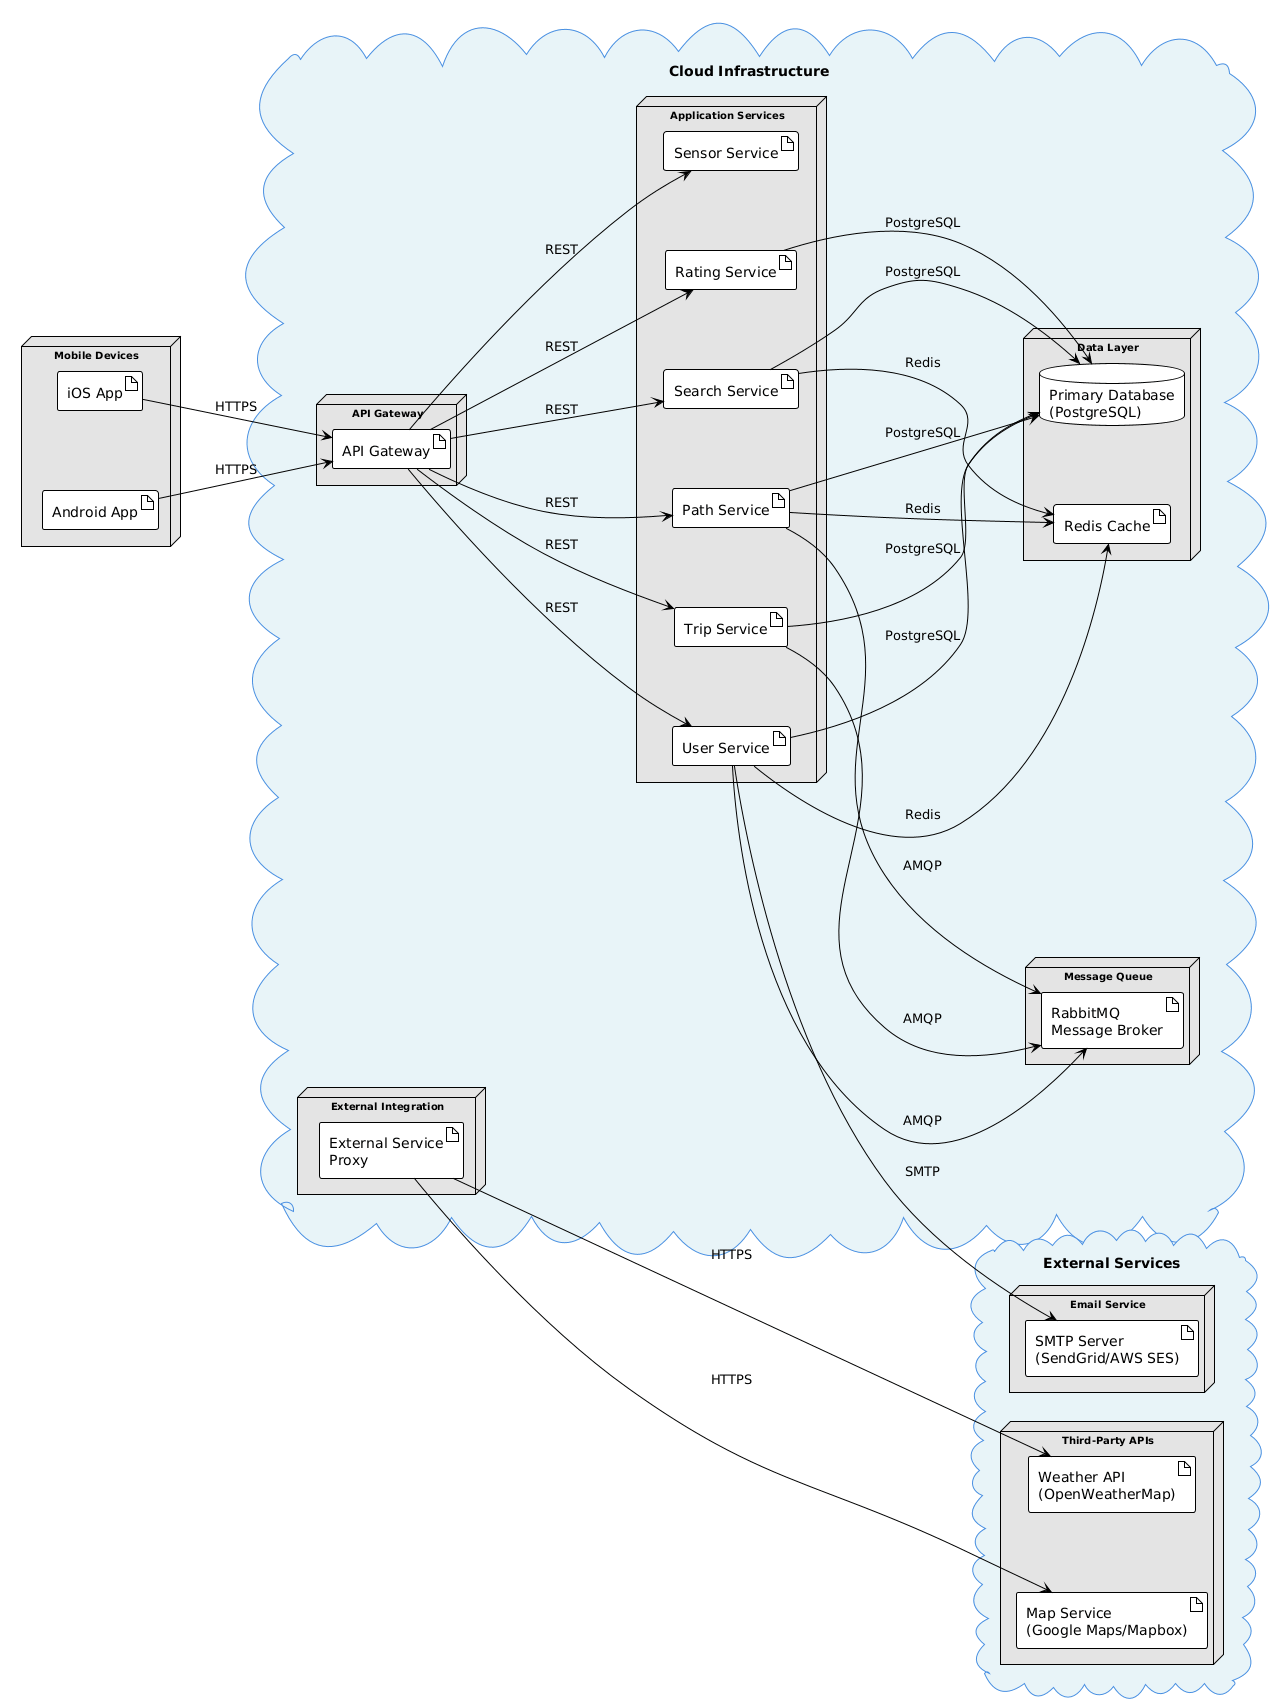
\includegraphics[width=0.95\linewidth]{Images/Diagrams/DeploymentViewDiagram.png}
        \caption{Deployment Diagram for Best Bike Paths System}
        \label{fig:deployment_diagram}%
    \end{center}
\end{figure}

\subsection{Client Deployment}
Mobile applications are deployed on user devices and serve as the primary interface for users to interact with the BBP system:

\begin{itemize}
    \item \textbf{iOS Application:} The application is designed to run natively on iOS devices, providing optimal performance and access to device-specific features such as GPS, accelerometer, and gyroscope sensors. Users will be able to download and install the application directly from the App Store, ensuring they receive the latest version with updates and security patches.
    
    \item \textbf{Android Application:} Similar to the iOS version, it is designed to run natively on Android devices, providing full access to device sensors and capabilities. Users will be able to download and install the application directly from the Play Store, ensuring they receive the latest version with updates and security patches.
    
    \item \textbf{Communication:} Both applications communicate with the backend server infrastructure using the HTTPS protocol, ensuring secure and encrypted data transmission. The applications exchange data in JSON format, providing a platform-independent data structure that works seamlessly across both mobile platforms.
    
\end{itemize}

\subsection{Server Deployment}
Backend services are deployed on cloud infrastructure:

\subsubsection{Web Server Layer}
\begin{itemize}
    \item \textbf{API Gateway:} The API Gateway serves as the single entry point for all client requests, handling incoming HTTPS connections from mobile applications. It performs several critical functions including request routing based on URL paths, authentication and authorization validation using JWT tokens, request validation to ensure data format and required fields are present. By centralizing these concerns, the API Gateway simplifies the architecture and provides a consistent interface for clients.
\end{itemize}

\subsubsection{Application Server Layer}
\begin{itemize}
    \item \textbf{Microservices Architecture:} The system follows a microservices architecture where each service (User Management, Trip Management, Path Management, Path Search, Sensor Data Processing, and Rating Service) runs as an independent, containerized instance. Each service is responsible for a specific domain of functionality, ensuring clear separation of concerns and independent development and deployment capabilities.
    
    \item \textbf{Scalability:} Services are designed to be stateless and horizontally scalable, allowing additional instances to be added dynamically based on demand.
    
    \item \textbf{Communication Patterns:} Services communicate using two main patterns: synchronous REST API calls for immediate request-response interactions, and asynchronous message queues for background processing and event-driven communication.
\end{itemize}

\subsubsection{Message Queue Layer}
\begin{itemize}
    \item \textbf{Message Broker:} RabbitMQ message broker handles asynchronous communication between services.
    
    \item \textbf{Protocol:} Services communicate using the AMQP (Advanced Message Queuing Protocol) protocol.
    
    \item \textbf{Use Cases:} The message queue is used for various asynchronous operations including sensor data processing, event notifications, and background job execution.
    
    \item \textbf{Benefits:} The message queue architecture improves system responsiveness by allowing services to respond immediately to user requests while deferring heavy processing.
\end{itemize}

\subsubsection{Data Layer}
\begin{itemize}
    \item \textbf{Primary Database:} PostgreSQL serves as the main database server for all persistent data operations, storing user profiles, authentication credentials, trip records, path information, obstacles, ratings, and system configuration.
    
    \item \textbf{Cache Layer:} Redis provides an in-memory caching layer that stores frequently accessed data to reduce database load and improve response times. The cache is used for storing session tokens, frequently searched path results, popular route information, and user profile data.
\end{itemize}

\subsubsection{External Services}
\begin{itemize}
    \item \textbf{Weather API:} Third-party weather service (e.g., OpenWeatherMap) provides meteorological data to enrich trip records.
    
    \item \textbf{Map Service:} Third-party mapping service (e.g., Google Maps, Mapbox) provides geographic data and visualization capabilities. The system uses map services to display routes on interactive maps in the mobile application, perform geocoding, and visualize path information including obstacles and route conditions.
    
    \item \textbf{Email Service:} SMTP server (e.g., SendGrid, AWS SES) handles all email communications including user account verification emails, password recovery emails, and system notifications.
\end{itemize}

\subsection{Infrastructure Specifications}

\subsubsection{Cloud Infrastructure}
The backend services are deployed on cloud infrastructure (AWS, Azure, or Google Cloud Platform) with the following characteristics:

\begin{itemize}
    \item \textbf{Containerization:} Services are containerized using Docker for consistent deployment across environments
    \item \textbf{Orchestration:} Docker Compose for prototype deployment. Kubernetes or Docker Swarm can be used for production environments requiring advanced orchestration features
    \item \textbf{Deployment:} One instance per service for the prototype. Services are designed to support horizontal scaling by adding more instances when needed in production
\end{itemize}

\subsubsection{Server Specifications}
Server specifications depend on the deployment environment and expected load. For the prototype, services can run on standard cloud instances with adequate resources. Typical requirements:

\begin{itemize}
    \item \textbf{Application Services:} Servers with sufficient CPU and RAM to run containerized services 
    \item \textbf{Storage:} SSD storage for logs and temporary data 
    \item \textbf{Network:} High-bandwidth network connection for efficient service communication
\end{itemize}

\subsubsection{Database Infrastructure}
Database server specifications:

\begin{itemize}
    \item \textbf{Primary Database:} PostgreSQL database server with adequate resources for data storage and query processing. Storage capacity depends on data volume and growth projections
    \item \textbf{Backup Strategy:} Automated backups on a regular schedule with point-in-time recovery capability to ensure data protection
\end{itemize}

\subsubsection{Cache Infrastructure}
Cache layer specifications:

\begin{itemize}
    \item \textbf{Technology:} Redis for in-memory caching
    \item \textbf{Configuration:} Standalone Redis instance for the prototype. Redis Cluster or Sentinel can be used in production for high availability
    \item \textbf{TTL Policy:} Default 1 hour time-to-live, configurable per key based on data freshness requirements
    \item \textbf{Eviction Policy:} Least Recently Used (LRU) policy to manage memory when cache is full
\end{itemize}

\subsection{Network Architecture}

\subsubsection{Network Topology}
\begin{itemize}
    \item \textbf{Public Network:} Clients connect via public internet to the API Gateway using HTTPS
    \item \textbf{Private Network:} Internal services communicate via private network to ensure security and isolation
    \item \textbf{Security:} Firewall rules and security groups restrict access:
    \begin{itemize}
        \item API Gateway: Accepts HTTPS from internet, forwards to services via HTTP
        \item Application Services: Accept REST API calls from API Gateway only
        \item Database: Accepts PostgreSQL connections from Application Services only
        \item Cache: Accepts Redis connections from Application Services only
    \end{itemize}
\end{itemize}

\subsubsection{Communication Protocols}
\begin{itemize}
    \item \textbf{Client to Server:} HTTPS
    \item \textbf{Internal Services:} HTTP/REST
    \item \textbf{Database:} PostgreSQL protocol
    \item \textbf{Cache:} Redis protocol
    \item \textbf{Message Queue:} AMQP protocol
    \item \textbf{Email:} SMTP
\end{itemize}

\subsection{High Availability and Scalability}

\subsubsection{High Availability Strategy}
For the prototype, the system focuses on core functionality with basic high availability measures:

\begin{itemize}
    \item \textbf{Service Design:} Services are designed to be stateless and horizontally scalable, allowing additional instances to be added when needed
    \item \textbf{Disaster Measures:} Automated database backups with point in time recovery capability to protect against data loss
\end{itemize}

\subsubsection{Scalability Strategy}
The system is designed with scalability in mind:

\begin{itemize}
    \item \textbf{Horizontal Scaling:} Services are stateless and can scale horizontally by adding more instances as demand increases
    \item \textbf{Database Scaling:} Vertical scaling (increasing resources) for the primary database. Read replicas can be added in production for read-heavy workloads
    \item \textbf{Cache Scaling:} Redis can be scaled horizontally using cluster mode in production environments
    \item \textbf{Production Scaling:} For production, auto-scaling policies can be configured based on metrics such as CPU utilization, request rate, or response time
\end{itemize}

\subsection{Monitoring and Logging}

For the prototype, basic monitoring and logging are implemented:

\begin{itemize}
    \item \textbf{Application Logging:} Services generate logs for analysis and debugging
    \item \textbf{Log Storage:} Logs are stored locally or in cloud storage for analysis and debugging
    \item \textbf{Basic Monitoring:} System health can be monitored through application logs and basic health check endpoints
\end{itemize}

\section{Runtime View}
\label{sec:runtime_view}%

The runtime view describes how components interact during the execution of specific use cases. The following sequence diagrams illustrate the flow of messages between the main client and server components for the majority of the defined use cases. To avoid redundancy, the data retrieval required to load the main page is shown in the login/registration interaction and then reused implicitly in the other interactions whenever the client needs to refresh the same data (e.g., map, nearby paths, past trips, and past reviews).

\subsection{User Login and Registration (UC1 \& UC2)}

\begin{figure}[H]
    \begin{center}
        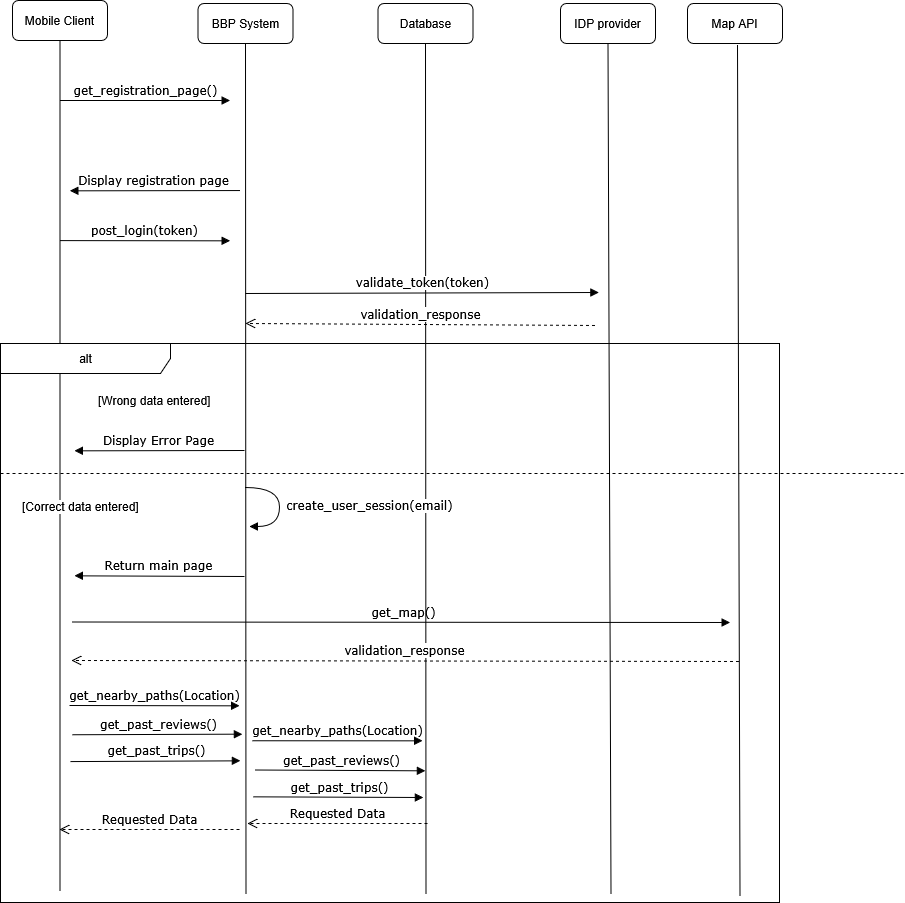
\includegraphics[width=0.95\linewidth]{Images/Diagrams/User_login.png}
        \caption{Sequence diagram for user login and registration (UC1 \& UC2)}
        \label{fig:seq_login_registration}
    \end{center}
\end{figure}

This sequence diagram represents the flow when a user logs into the BBP system. First, the login/register page is shown. When the user selects login, the client sends an IDP token to the system, which forwards it to the IDP to validate the credentials. If validation fails, the user is shown an error page; if it succeeds, the user is redirected to the main page and the client requests the data that is not stored locally (map, nearby paths, past trips, and past reviews).

The registration flow is analogous: the user also provides basic profile data to be stored in the DBMS, and the system confirms that the email is not already registered.

\subsection{Enter Path Manually (UC3 \& UC5)}

\begin{figure}[H]
    \begin{center}
        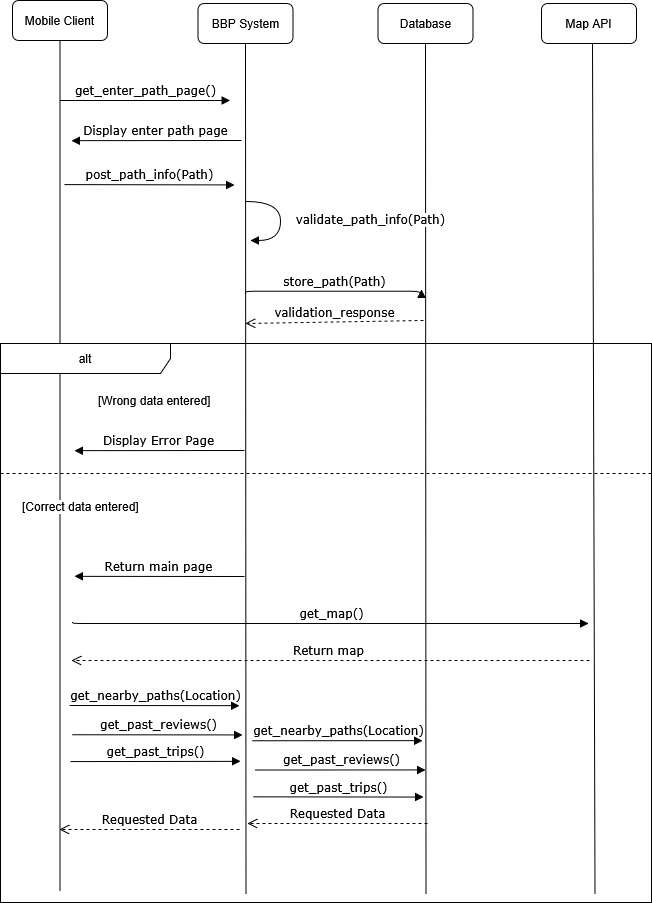
\includegraphics[width=0.95\linewidth]{Images/Diagrams/enter_path_manually.png}
        \caption{Sequence diagram for manual path entry and publishing (UC3 \& UC5)}
        \label{fig:seq_enter_path_manually}
    \end{center}
\end{figure}

The diagram includes use cases UC3 and UC5. First, the user enters the data for a new path; the system validates and parses it. If the data is correct and the path does not already exist, it is stored in the database. If the user chooses to publish it, the same validated data is made available to other users through the path management and search functionalities.

\subsection{Detect Path Automatically (UC4)}

\begin{figure}[H]
    \begin{center}
        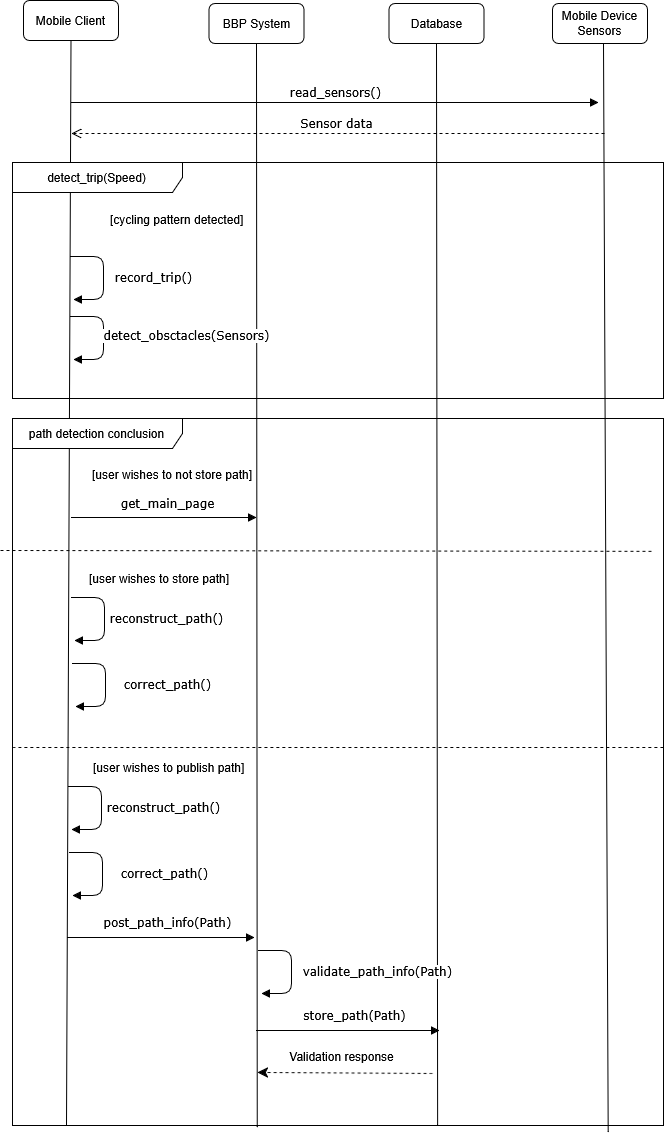
\includegraphics[width=0.75\linewidth, keepaspectratio=true]{Images/Diagrams/detect_path_automatically.png}
        \caption{Sequence diagram for automatic path detection (UC4)}
        \label{fig:seq_detect_path_automatically}
    \end{center}
\end{figure}

To detect trips automatically, the client accesses the sensors of the mobile device and monitors when speed reaches a threshold (above running speed and below driving speed). When the threshold is crossed, the system prompts the user (when opening the app) with the detected path data. The user can discard it, store it locally, or publish it. If it is stored locally, the user confirms the information; if it is published, the user can correct it first and then the publication flow follows the same interaction described in UC5.

\subsection{Search and Visualize Paths Between Two Points (UC6)}

\begin{figure}[H]
    \begin{center}
        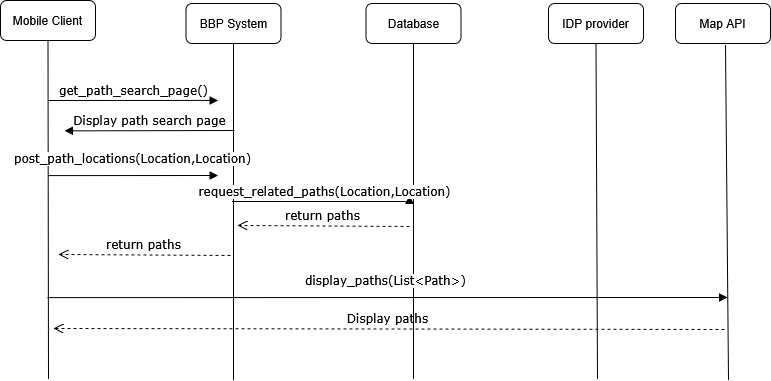
\includegraphics[width=0.95\linewidth]{Images/Diagrams/search_visualize_between_two_points.png}
        \caption{Sequence diagram for searching and visualizing paths between two points (UC6)}
        \label{fig:seq_search_visualize}
    \end{center}
\end{figure}

When the user searches for paths between two points, they enter both locations and the system searches the database for related paths. Once the client obtains the list of possible paths, it uses the Map API to display them on the map.

\subsection{Post Review and Merge Information from Multiple Users (UC7 \& UC12)}

\begin{figure}[H]
    \begin{center}
        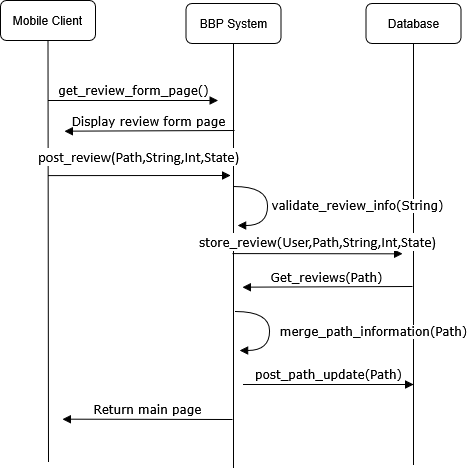
\includegraphics[width=0.95\linewidth]{Images/Diagrams/post_review_merge.png}
        \caption{Sequence diagram for posting reviews and merging information (UC7 \& UC12)}
        \label{fig:seq_post_review_merge}
    \end{center}
\end{figure}

To post a new review for a path, the user opens the path page and selects to add a review. The client displays the review form and, after submission, the data is sent to the server where it is validated and stored. After that, the system re-checks all reviews for the path to recalculate the overall score and update the most recent status. This refreshed information is then used by the information merging logic to consolidate updates coming from multiple users.

\subsection{See Path Data, Trip Statistics and Check Review (UC9, UC10 \& UC11)}

\begin{figure}[H]
    \begin{center}
        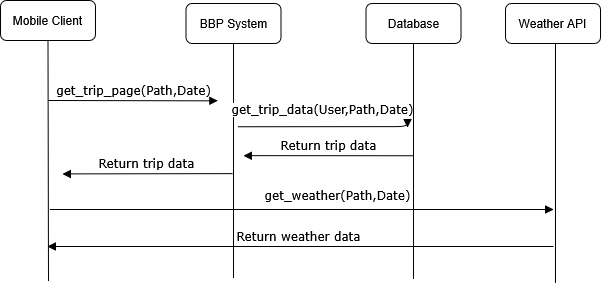
\includegraphics[width=0.95\linewidth]{Images/Diagrams/get_trip_data.png}
        \caption{Sequence diagram for retrieving path/trip/review data (UC9, UC10 \& UC11)}
        \label{fig:seq_get_trip_data}
    \end{center}
\end{figure}

These three use cases are similar: the user requests information for a specific item and the system retrieves it from the database. The main difference is in the trip statistics flow, where the Weather API is also accessed to enrich the trip data with meteorological information.

\section{Component Interfaces}
\label{sec:component_interfaces}%

This section lists the methods used in the interfaces of the systems, they attempt to be as straight-forward as possible. Even though fewer methods will be available for external components, all of them are listed here.
It is important to be noted that methods such as \texttt{get\_trip\_data} can be used internally in case the trip is stored in the client device, or can send a message to the system in case the trip has to be retrieved from the database. 

\begin{itemize}
    \item \textbf{userData}: user's name and optional profile picture.
    \item \textbf{token}: an IDP token used for authentication.
    \item \textbf{Location}: an \texttt{Int} \(\times\) \texttt{Int} tuple representing latitude and longitude.
    \item \textbf{Path}: an object including a \texttt{String} name, a starting \textbf{Location}, and two \texttt{Int} values for length (meters) and estimated duration (based on average biking speed).
\end{itemize}


\subsection{User Management Service Interface}
\begin{itemize}
    \item \texttt{get\_registration\_page()}
    \item \texttt{post\_register(token)}
    \item \texttt{post\_login(token)}
    \item \texttt{create\_user\_session(email)}
    \item \texttt{end\_user\_session(email)}
    \item \texttt{get\_user\_data()}
    \item \texttt{get\_past\_trips()}
    \item \texttt{get\_past\_reviews()}
\end{itemize}

\subsection{Trip Management Service Interface}
\begin{itemize}
 \item \texttt{detect\_trip(Speed)}
    \item \texttt{record\_trip()}
    \item \texttt{detect\_obstacles(Speed, sensor\_data)}
    \item \texttt{reconstruct\_path(List<Location>)}
    \item \texttt{correct\_path()}
    \item \texttt{post\_path\_locations(Location, Location)}
    \item \texttt{start\_trip(Path)}
    \item \texttt{end\_trip(Path)}
    \item \texttt{store\_trip(Path, Date)}
    \item \texttt{get\_trip\_page()}
    \item \texttt{get\_trip\_data(User, Path, Date)}
\end{itemize}

\subsection{Path Management Service Interface}
\begin{itemize}
    \item \texttt{get\_nearby\_paths(Location)}
    \item \texttt{get\_enter\_path\_page()}
    \item \texttt{post\_path\_info(Path)}
    \item \texttt{validate\_path\_info(Path)}
    \item \texttt{validate\_review\_info(String)}
    \item \texttt{request\_related\_paths(Location, Location)}
    \item \texttt{display\_paths(List<Path>)}
    \item \texttt{get\_path\_search\_page()}
    \item \texttt{add\_path(List<Location>, List<String>)}
    \item \texttt{get\_reviews(Path)}
    \item \texttt{merge\_path\_information(Path)}
    \item \texttt{post\_path\_update(Path)}
    \item \texttt{get\_path\_page(Path)}
    \item \texttt{get\_path\_data(Path)}
\end{itemize}

\subsection{Rating Service Interface}
\begin{itemize}
    \item \texttt{get\_review\_form\_page()}
    \item \texttt{post\_review(Path, String, Int, State)}
    \item \texttt{get\_review\_page(Path)}
    \item \texttt{get\_review\_data(Path, User, Date)}
\end{itemize}

\subsection{DBMS Interface}
\begin{itemize}
    \item \texttt{store\_review(User, Path, String, Int, State)}
    \item \texttt{store\_path(Path)}
\end{itemize}

\subsection{Accelerometer \& Gyroscope}
\begin{itemize}
    \item \texttt{read\_sensors()}
\end{itemize}

\subsection{Map API}
\begin{itemize}
    \item \texttt{get\_map(Location)}
\end{itemize}

\subsection{Weather API}
\begin{itemize}
    \item \texttt{get\_weather(Date, Path)}
\end{itemize}

\subsection{IDP}
\begin{itemize}
    \item \texttt{validate\_token(token)}
\end{itemize}

\section{Selected Architectural Styles and Patterns}
\label{sec:architectural_styles_patterns}%

\subsection{Architectural Styles}

\subsubsection{Client-Server Architecture}

The system adopts a client--server architecture in which each mobile application operates as a client that sends requests to backend servers. The server side is responsible for centralized business logic execution and shared data management, ensuring data consistency among users, reducing computation on client devices, and avoiding data duplication across clients.

\subsubsection{Layered Architecture}

The system is organized in layers. The presentation layer corresponds to the frontend mobile application used by clients. The application layer manages the core logic services and coordinates the execution of use cases. The data layer consists of the database management system, which is accessed exclusively through repositories, as described later. This structure improves separation of concerns and maintainability.

\subsubsection{Model-View-Controller (MVC)}

On the client side, the Model–View–Controller pattern is adopted to structure the mobile application. The model represents the data structures and application logic, the view includes all user interface components, and the controller manages user input and coordinates interactions between the model and the view. This pattern improves modularity and simplifies the evolution of the user interface.

\subsubsection{Microservices Architecture}

Backend services such as user management, trip management, etc, are organized as microservices, where each of them is independently deployable and isolated, benefiting scalability, testing and independent development.

\subsubsection{Repository Pattern}
The repository pattern is used to abstract data access and centralize all database retrieval and storage operations. By isolating persistence-related code from domain and application logic, this pattern improves testability and supports flexibility in case of future changes to the database technology.


\subsubsection{Facade Pattern}
The facade pattern is employed to provide simplified interfaces to the application services exposed by the backend. These facades encapsulate the complexity of the underlying components and repositories, reducing coupling and simplifying the interaction between the mobile application controllers and the server-side logic.

\subsubsection{Observer Pattern}

The observer pattern is used on the client side to support event-driven processing of sensor data. Components responsible for acquiring data from the gyroscope and accelerometer act as subjects, notifying observer components when relevant events occur. This enables efficient detection of trips and potholes while maintaining loose coupling between sensor data acquisition and processing logic.

\section{Other Design Decisions}
\label{sec:other_design_decisions}%

\subsection{Offline Support}

The mobile application provides basic offline support to improve usability in scenarios with limited or no network connectivity. The client is able to locally cache nearby map data and bike paths, as well as record trips while offline. Once connectivity is restored, locally stored data is synchronized with the backend servers. This design improves robustness and user experience in mobile usage contexts.


\subsection{Security}

All communications between the client and backend services are performed over HTTPS to ensure confidentiality and integrity of transmitted data. Authentication is implemented using token-based mechanisms, allowing stateless and secure session management. If credential management is handled by the system, user passwords are never stored in plain text and are securely hashed using industry-standard algorithms such as bcrypt.

\subsection{Performance Optimization}
Performance optimizations include:
\begin{itemize}
    \item Database indexing for frequent queries
    \item Caching of frequently accessed data
    \item Lazy loading of map data
    \item Efficient sensor data processing algorithms
    \item Battery optimization for continuous sensor monitoring
\end{itemize}

\subsection{Error Handling}

The system is designed to support graceful degradation in the presence of partial failures or unavailable services. When errors occur, the user is presented with clear and understandable error messages. On the server side, errors are logged and monitored to support diagnosis and maintenance. Retry mechanisms are implemented where appropriate, with controlled limits to avoid cascading failures.
